\documentclass[12pt,addpoints]{exam}
\usepackage{amsmath,amssymb} % standard math extensions
\usepackage{tikz} % for graphs and figures
%\usepackage{pgfplots}
%\pgfplotsset{width=10cm,compat=1.9}
\usepackage{graphicx} % for including the JAC logo

% change the following five definitions as needed
\newcommand{\Date}{26 May 2025}
\newcommand{\Time}{{\upshape 9h--12h}}
\newcommand{\Course}{Calculus II}
\newcommand{\CourseNumber}{201-NYB-05}
\newcommand{\Instructors}{Jason Lucier, Yu Zhao}

% exam document class formatting commands
\extrawidth{1in}
\extraheadheight{-0.25in}
\extrafootheight{-0.375in}
\renewcommand{\questionlabel}{\bfseries\thequestion.} % bold question numbers
\pagestyle{headandfoot}
\lhead{Final Examination}
\chead{\CourseNumber}
\rhead{\Date}
\headrule 
\lfoot{\iflastpage{Total: \numpoints~points}{}}
\cfoot{Page \thepage\ of \numpages}
\rfoot{\iflastpage{This is the end of the examination.}{%
  \ifincomplete{%
    Question~{\IncompleteQuestion} continues on the next page.}{%
    Please go on to the next page.}}}

% install fonts for the title page
\usepackage{oldgerm}
\newfont{\yinit}{yinit at 45pt}
\def\yinitial#1{
\hskip-2mm
\lower2mm
\hbox{\yinit #1}
\hskip-2mm}

% math commands
\newcommand{\reals}{\mathbb{R}} % use blackboard bold for the real numbers
\renewcommand{\le}{\leqslant} % another style of 'less than or equal to'
\renewcommand{\ge}{\geqslant} % another style of 'greater than or equal to'
\newcommand{\dsp}{\displaystyle} % a convenient abbreviation

\everymath{\displaystyle}
\begin{document}



\begin{questions}
% Use optional arguments to \question and \part to state mark values.
% Add \vspace after each question or part as needed.

\question Evaluate the following integrals. 
\begin{parts}
\part[5] $\int x\sqrt{x+5}\,dx$

\part[5] $\int \frac{x-2}{x^2+6x+25}\,dx$

\part[5] $\int x\cos\left(2x/5\right)\,dx$

\part[5] $\int_0^{5/2} \frac{x^2}{\sqrt{25-x^2}}\,dx$

\part[5] $\int \tan^2(x)\sec^4(x)\,dx$ 

\part[5] $\int \frac{1}{e^x(e^{2x}+1)}\,dx$
\end{parts}

\question Evaluate the following limits. 
\begin{parts}
\part[4] $\lim_{x \to 0} \frac{x-2\arctan(x)}{x+5\arcsin(x)}$

\part[4] $\lim_{x \to \infty} \left( \sec\left(\frac{5}{x}\right)\right)^{x^2}$
\end{parts}

\question Evaluate each improper integral or show it diverges. 
\begin{parts}
\part[5] $\int_1^e \frac{dx}{x\ln(x)}$

\part[5] $\int_1^\infty \frac{dx}{x(2x+5)}$
\end{parts}

\begin{minipage}[t]{0.55\textwidth}
\question[4] Find the area of the region bounded by the curves given by $y=\frac{1}{x+1}$ and $y=\frac{1}{x^2+1}$.
\end{minipage}
\begin{minipage}[t]{0.4\textwidth}
\begin{center}
\begin{tikzpicture}[baseline=(current bounding box.north),scale=1.1]
\draw[->] (-1,0)--(2.25,0) node [right] {$x$};
\draw[->] (0,-0.25)--(0,2.25) node [above] {$y$};
\draw[domain=-0.55:2, smooth] plot ({\x}, {1/(\x+1)});
\draw[domain=-0.75:2, smooth] plot ({\x}, {1/(\x*\x+1)});
\end{tikzpicture}
\end{center}
\end{minipage}

\question[5] Solve the differential equation $\frac{dy}{dx} = y^2\ln(x)$ with $y(1)=-1$. 

\begin{minipage}[t]{0.55\textwidth}
\question In the figure a shaded rectangle is divided into two regions, $R_1$ and $R_2$, by the curve $y=1-x^2$. 
Write down, \textsl{but do not evaluate}, an integral for the volume of the solid of revolution obtained by 
\vspace{5pt}
\begin{parts}
\part[2] rotating $R_1$ about the $x$-axis

\part[2] rotating $R_1$ about the line $y=2$

\part[2] rotating $R_2$ about the line $x=2$.
\end{parts}
\end{minipage}
\begin{minipage}[t]{0.4\textwidth}
\begin{center}
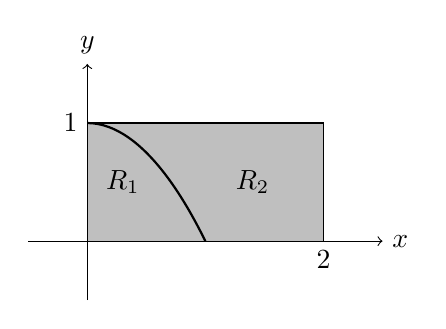
\begin{tikzpicture}[baseline=(current bounding box.north),scale = 1.5]
\draw[->] (-0.5,0) -- (2.5,0) node[right] {$x$};
\draw[->] (0,-0.5) -- (0,1.5) node[above] {$y$};
\node at (0,1) [left] {$1$};
\node at (2,0) [below] {$2$};
\filldraw[fill=gray!50!white] (0,0) rectangle (2,1);
\draw[thick] (0,1) parabola (1,0);
\node at (0.3,0.5) [] {$R_1$};
\node at (1.4,0.5) [] {$R_2$};
\end{tikzpicture}
\end{center}
\end{minipage}

\question[5] Find the length of the curve given by $y=\sqrt{4-x^2}$ for $0 \leq x \leq 1$.

\question[3] Determine the sum of the series $\sum_{n=1}^\infty \frac{2+5^n}{5^{2n}}$.

\question Determine whether the series converges or diverges.
\begin{parts}
\part[3] $\sum_{n=1}^\infty \frac{\arctan(n)}{n}$ 

\part[3] $\sum_{n=0}^\infty \frac{2^n}{5^n+n}$ 

\part[3] $\sum_{n=1}^\infty n^2\sin\left(\frac{1}{n^5}\right)$ 
\end{parts}

\question Determine whether the series converges absolutely, converges conditionally, or diverges. 
\begin{parts}
\part[3] $\sum_{n=1}^\infty (-1)^n \frac{n+2}{n+5}$ 

\part[3] $\sum_{n=1}^\infty \frac{(-1)^n}{\sqrt{n^2+1}}$ 

\part[3] $\sum_{n=0}^\infty (-1)^n\frac{(2n+1)!}{5^n(n!)^2}$
\end{parts}

\question[5] Find the interval of convergence of the power series $\sum_{n=1}^\infty \frac{(-1)^n}{2^n n}(x+1)^n$. 

\question[5] Find the Taylor series for $f(x) = \frac{1}{(x+1)^2}$ centred at $4$. Give your answer using sigma notation.

\question[1] If $f(x) = \sum_{n=1}^\infty \frac{\cos(n\pi/2)}{n^2}x^n$, what is the coefficient of $x^{25}$ in the Maclaurin series for $f'(x)$? 
\end{questions}

\newpage
{\small
\textbf{Answers:}

\begin{questions}
% Use optional arguments to \question and \part to state mark values.
% Add \vspace after each question or part as needed.

\question 
\begin{parts}
\part $\frac{2}{5}(x+5)^{5/2}-\frac{10}{3}(x+5)^{3/2} +C$ 

\part $\frac{1}{2}\ln(x^2+6x+25)-\frac{5}{4}\arctan\left(\frac{x+3}{4}\right)+C$

\part $\frac{5}{2}x\sin\left(\frac{2x}{5}\right)+ \frac{25}{4}\cos\left(\frac{2x}{5}\right)+C$

\part $\frac{25}{24}(2\pi-3\sqrt{3})$

\part $\frac{1}{3}\tan^3(x)+\frac{1}{5}\tan^5(x)+C$ 

\part $-e^{-x}-\tan(e^x)+C$
\end{parts}

\question  
\begin{parts}
\part $-\frac{1}{6}$

\part $e^{25/2}$
\end{parts}

\question 
\begin{parts}
\part diverges (to $\infty$)

\part $\frac{1}{5}\ln\left(\frac{7}{2}\right)$
\end{parts}

\question $\frac{\pi}{4}-\ln(2)$ 

\question $y=-\frac{1}{x\ln(x)-x+2} $. 

\question 
\begin{parts}
\part $\int_0^1 \pi(1-x^2)^2dx$ or $\int_0^1 2\pi y\sqrt{1-y}dy$ 

\part $\int_0^1\pi[4-(1+x^2)^2]dx$ or $\int_0^1 2\pi(2-y)\sqrt{1-y}dy$

\part $\int_0^1 \pi(2-\sqrt{1-y})^2dy$
\end{parts}


\question $\frac{\pi}{3}$

\question $\frac{1}{3}$

\question 
\begin{parts}
\part diverges 

\part converges

\part converges
\end{parts}

\question 
\begin{parts}
\part diverges

\part converges conditionally

\part converges absolutely 
\end{parts}

\question $(-3,1]$

\question $\sum_{n=0}^\infty \frac{(-1)^n(n+1)}{5^{n+2}}(x-4)^n$

\question $-\frac{1}{26}$ 
\end{questions}
}
\end{document}
